\documentclass[1p]{elsarticle_modified}
%\bibliographystyle{elsarticle-num}

%\usepackage[colorlinks]{hyperref}
%\usepackage{abbrmath_seonhwa} %\Abb, \Ascr, \Acal ,\Abf, \Afrak
\usepackage{amsfonts}
\usepackage{amssymb}
\usepackage{amsmath}
\usepackage{amsthm}
\usepackage{scalefnt}
\usepackage{amsbsy}
\usepackage{kotex}
\usepackage{caption}
\usepackage{subfig}
\usepackage{color}
\usepackage{graphicx}
\usepackage{xcolor} %% white, black, red, green, blue, cyan, magenta, yellow
\usepackage{float}
\usepackage{setspace}
\usepackage{hyperref}

\usepackage{tikz}
\usetikzlibrary{arrows}

\usepackage{multirow}
\usepackage{array} % fixed length table
\usepackage{hhline}

%%%%%%%%%%%%%%%%%%%%%
\makeatletter
\renewcommand*\env@matrix[1][\arraystretch]{%
	\edef\arraystretch{#1}%
	\hskip -\arraycolsep
	\let\@ifnextchar\new@ifnextchar
	\array{*\c@MaxMatrixCols c}}
\makeatother %https://tex.stackexchange.com/questions/14071/how-can-i-increase-the-line-spacing-in-a-matrix
%%%%%%%%%%%%%%%

\usepackage[normalem]{ulem}

\newcommand{\msout}[1]{\ifmmode\text{\sout{\ensuremath{#1}}}\else\sout{#1}\fi}
%SOURCE: \msout is \stkout macro in https://tex.stackexchange.com/questions/20609/strikeout-in-math-mode

\newcommand{\cancel}[1]{
	\ifmmode
	{\color{red}\msout{#1}}
	\else
	{\color{red}\sout{#1}}
	\fi
}

\newcommand{\add}[1]{
	{\color{blue}\uwave{#1}}
}

\newcommand{\replace}[2]{
	\ifmmode
	{\color{red}\msout{#1}}{\color{blue}\uwave{#2}}
	\else
	{\color{red}\sout{#1}}{\color{blue}\uwave{#2}}
	\fi
}

\newcommand{\Sol}{\mathcal{S}} %segment
\newcommand{\D}{D} %diagram
\newcommand{\A}{\mathcal{A}} %arc


%%%%%%%%%%%%%%%%%%%%%%%%%%%%%5 test

\def\sl{\operatorname{\textup{SL}}(2,\Cbb)}
\def\psl{\operatorname{\textup{PSL}}(2,\Cbb)}
\def\quan{\mkern 1mu \triangleright \mkern 1mu}

\theoremstyle{definition}
\newtheorem{thm}{Theorem}[section]
\newtheorem{prop}[thm]{Proposition}
\newtheorem{lem}[thm]{Lemma}
\newtheorem{ques}[thm]{Question}
\newtheorem{cor}[thm]{Corollary}
\newtheorem{defn}[thm]{Definition}
\newtheorem{exam}[thm]{Example}
\newtheorem{rmk}[thm]{Remark}
\newtheorem{alg}[thm]{Algorithm}

\newcommand{\I}{\sqrt{-1}}
\begin{document}

%\begin{frontmatter}
%
%\title{Boundary parabolic representations of knots up to 8 crossings}
%
%%% Group authors per affiliation:
%\author{Yunhi Cho} 
%\address{Department of Mathematics, University of Seoul, Seoul, Korea}
%\ead{yhcho@uos.ac.kr}
%
%
%\author{Seonhwa Kim} %\fnref{s_kim}}
%\address{Center for Geometry and Physics, Institute for Basic Science, Pohang, 37673, Korea}
%\ead{ryeona17@ibs.re.kr}
%
%\author{Hyuk Kim}
%\address{Department of Mathematical Sciences, Seoul National University, Seoul 08826, Korea}
%\ead{hyukkim@snu.ac.kr}
%
%\author{Seokbeom Yoon}
%\address{Department of Mathematical Sciences, Seoul National University, Seoul, 08826,  Korea}
%\ead{sbyoon15@snu.ac.kr}
%
%\begin{abstract}
%We find all boundary parabolic representation of knots up to 8 crossings.
%
%\end{abstract}
%\begin{keyword}
%    \MSC[2010] 57M25 
%\end{keyword}
%
%\end{frontmatter}

%\linenumbers
%\tableofcontents
%
\newcommand\colored[1]{\textcolor{white}{\rule[-0.35ex]{0.8em}{1.4ex}}\kern-0.8em\color{red} #1}%
%\newcommand\colored[1]{\textcolor{white}{ #1}\kern-2.17ex	\textcolor{white}{ #1}\kern-1.81ex	\textcolor{white}{ #1}\kern-2.15ex\color{red}#1	}

{\Large $\underline{12a_{1269}~(K12a_{1269})}$}

\setlength{\tabcolsep}{10pt}
\renewcommand{\arraystretch}{1.6}
\vspace{1cm}\begin{tabular}{m{100pt}>{\centering\arraybackslash}m{274pt}}
\multirow{5}{120pt}{
	\centering
	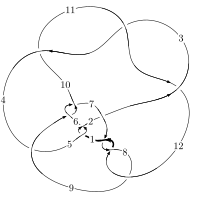
\includegraphics[width=112pt]{../../../GIT/diagram.site/Diagrams/png/2070_12a_1269.png}\\
\ \ \ A knot diagram\footnotemark}&
\allowdisplaybreaks
\textbf{Linearized knot diagam} \\
\cline{2-2}
 &
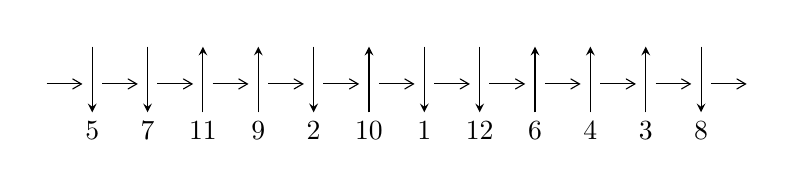
\begin{tikzpicture}[x=20pt, y=17pt]
	% nodes
	\node (C0) at (0, 0) {};
	\node (C1) at (1, 0) {};
	\node (C1U) at (1, +1) {};
	\node (C1D) at (1, -1) {5};

	\node (C2) at (2, 0) {};
	\node (C2U) at (2, +1) {};
	\node (C2D) at (2, -1) {7};

	\node (C3) at (3, 0) {};
	\node (C3U) at (3, +1) {};
	\node (C3D) at (3, -1) {11};

	\node (C4) at (4, 0) {};
	\node (C4U) at (4, +1) {};
	\node (C4D) at (4, -1) {9};

	\node (C5) at (5, 0) {};
	\node (C5U) at (5, +1) {};
	\node (C5D) at (5, -1) {2};

	\node (C6) at (6, 0) {};
	\node (C6U) at (6, +1) {};
	\node (C6D) at (6, -1) {10};

	\node (C7) at (7, 0) {};
	\node (C7U) at (7, +1) {};
	\node (C7D) at (7, -1) {1};

	\node (C8) at (8, 0) {};
	\node (C8U) at (8, +1) {};
	\node (C8D) at (8, -1) {12};

	\node (C9) at (9, 0) {};
	\node (C9U) at (9, +1) {};
	\node (C9D) at (9, -1) {6};

	\node (C10) at (10, 0) {};
	\node (C10U) at (10, +1) {};
	\node (C10D) at (10, -1) {4};

	\node (C11) at (11, 0) {};
	\node (C11U) at (11, +1) {};
	\node (C11D) at (11, -1) {3};

	\node (C12) at (12, 0) {};
	\node (C12U) at (12, +1) {};
	\node (C12D) at (12, -1) {8};
	\node (C13) at (13, 0) {};

	% arrows
	\draw[->,>={angle 60}]
	(C0) edge (C1) (C1) edge (C2) (C2) edge (C3) (C3) edge (C4) (C4) edge (C5) (C5) edge (C6) (C6) edge (C7) (C7) edge (C8) (C8) edge (C9) (C9) edge (C10) (C10) edge (C11) (C11) edge (C12) (C12) edge (C13) ;	\draw[->,>=stealth]
	(C1U) edge (C1D) (C2U) edge (C2D) (C3D) edge (C3U) (C4D) edge (C4U) (C5U) edge (C5D) (C6D) edge (C6U) (C7U) edge (C7D) (C8U) edge (C8D) (C9D) edge (C9U) (C10D) edge (C10U) (C11D) edge (C11U) (C12U) edge (C12D) ;
	\end{tikzpicture} \\
\hhline{~~} \\& 
\textbf{Solving Sequence} \\ \cline{2-2} 
 &
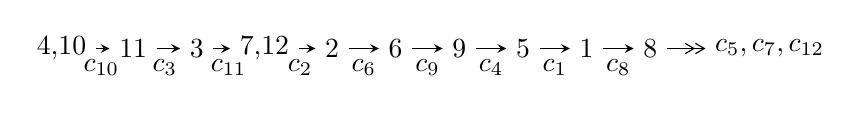
\begin{tikzpicture}[x=23pt, y=7pt]
	% node
	\node (A0) at (-1/8, 0) {4,10};
	\node (A1) at (1, 0) {11};
	\node (A2) at (2, 0) {3};
	\node (A3) at (49/16, 0) {7,12};
	\node (A4) at (33/8, 0) {2};
	\node (A5) at (41/8, 0) {6};
	\node (A6) at (49/8, 0) {9};
	\node (A7) at (57/8, 0) {5};
	\node (A8) at (65/8, 0) {1};
	\node (A9) at (73/8, 0) {8};
	\node (C1) at (1/2, -1) {$c_{10}$};
	\node (C2) at (3/2, -1) {$c_{3}$};
	\node (C3) at (5/2, -1) {$c_{11}$};
	\node (C4) at (29/8, -1) {$c_{2}$};
	\node (C5) at (37/8, -1) {$c_{6}$};
	\node (C6) at (45/8, -1) {$c_{9}$};
	\node (C7) at (53/8, -1) {$c_{4}$};
	\node (C8) at (61/8, -1) {$c_{1}$};
	\node (C9) at (69/8, -1) {$c_{8}$};
	\node (A10) at (11, 0) {$c_{5},c_{7},c_{12}$};

	% edge
	\draw[->,>=stealth]	
	(A0) edge (A1) (A1) edge (A2) (A2) edge (A3) (A3) edge (A4) (A4) edge (A5) (A5) edge (A6) (A6) edge (A7) (A7) edge (A8) (A8) edge (A9) ;
	\draw[->>,>={angle 60}]	
	(A9) edge (A10);
\end{tikzpicture} \\ 

\end{tabular} \\

\footnotetext{
The image of knot diagram is generated by the software ``\textbf{Draw programme}" developed by Andrew Bartholomew(\url{http://www.layer8.co.uk/maths/draw/index.htm\#Running-draw}), where we modified some parts for our purpose(\url{https://github.com/CATsTAILs/LinksPainter}).
}\phantom \\ \newline 
\centering \textbf{Ideals for irreducible components\footnotemark of $X_{\text{par}}$} 
 
\begin{align*}
I^u_{1}&=\langle 
5.85714\times10^{181} u^{95}+9.69877\times10^{181} u^{94}+\cdots+1.18195\times10^{183} b+3.37065\times10^{183},\\
\phantom{I^u_{1}}&\phantom{= \langle  }2.93871\times10^{183} u^{95}-7.16174\times10^{183} u^{94}+\cdots+5.42517\times10^{185} a+2.14826\times10^{185},\\
\phantom{I^u_{1}}&\phantom{= \langle  }u^{96}+2 u^{95}+\cdots+252 u+36\rangle \\
I^u_{2}&=\langle 
b+1,\;3 a^2+4 a u-2 a+2 u-1,\;u^2- u+1\rangle \\
I^u_{3}&=\langle 
a u+17 b-10 a+2 u-3,\;6 a^2-3 a u-6 a+4 u+13,\;u^2+2\rangle \\
I^u_{4}&=\langle 
b-1,\;3 a+2 u+1,\;u^2+u+1\rangle \\
\\
I^v_{1}&=\langle 
a,\;b+3 v-2,\;3 v^2-3 v+1\rangle \\
\end{align*}
\raggedright * 5 irreducible components of $\dim_{\mathbb{C}}=0$, with total 108 representations.\\
\footnotetext{All coefficients of polynomials are rational numbers. But the coefficients are sometimes approximated in decimal forms when there is not enough margin.}
\newpage
\renewcommand{\arraystretch}{1}
\centering \section*{I. $I^u_{1}= \langle 5.86\times10^{181} u^{95}+9.70\times10^{181} u^{94}+\cdots+1.18\times10^{183} b+3.37\times10^{183},\;2.94\times10^{183} u^{95}-7.16\times10^{183} u^{94}+\cdots+5.43\times10^{185} a+2.15\times10^{185},\;u^{96}+2 u^{95}+\cdots+252 u+36 \rangle$}
\flushleft \textbf{(i) Arc colorings}\\
\begin{tabular}{m{7pt} m{180pt} m{7pt} m{180pt} }
\flushright $a_{4}=$&$\begin{pmatrix}0\\u\end{pmatrix}$ \\
\flushright $a_{10}=$&$\begin{pmatrix}1\\0\end{pmatrix}$ \\
\flushright $a_{11}=$&$\begin{pmatrix}1\\- u^2\end{pmatrix}$ \\
\flushright $a_{3}=$&$\begin{pmatrix}- u\\u^3+u\end{pmatrix}$ \\
\flushright $a_{7}=$&$\begin{pmatrix}-0.00541682 u^{95}+0.0132010 u^{94}+\cdots+0.00687780 u-0.395980\\-0.0495547 u^{95}-0.0820571 u^{94}+\cdots-14.3667 u-2.85176\end{pmatrix}$ \\
\flushright $a_{12}=$&$\begin{pmatrix}u^2+1\\- u^4-2 u^2\end{pmatrix}$ \\
\flushright $a_{2}=$&$\begin{pmatrix}0.0992526 u^{95}-0.0551318 u^{94}+\cdots-32.0600 u-5.27325\\-0.0122200 u^{95}+0.0105278 u^{94}+\cdots-4.85256 u-1.05968\end{pmatrix}$ \\
\flushright $a_{6}=$&$\begin{pmatrix}0.0441379 u^{95}+0.0952581 u^{94}+\cdots+14.3735 u+2.45578\\-0.0495547 u^{95}-0.0820571 u^{94}+\cdots-14.3667 u-2.85176\end{pmatrix}$ \\
\flushright $a_{9}=$&$\begin{pmatrix}0.0234885 u^{95}+0.0658944 u^{94}+\cdots+3.68018 u+1.26869\\0.0283007 u^{95}+0.0420807 u^{94}+\cdots+8.03772 u+0.727400\end{pmatrix}$ \\
\flushright $a_{5}=$&$\begin{pmatrix}-0.00746047 u^{95}+0.233084 u^{94}+\cdots+48.9621 u+6.70772\\-0.0189892 u^{95}-0.0718124 u^{94}+\cdots-16.8541 u-3.26791\end{pmatrix}$ \\
\flushright $a_{1}=$&$\begin{pmatrix}0.000359993 u^{95}+0.0337391 u^{94}+\cdots-1.28875 u+0.181747\\-0.0229557 u^{95}-0.0459877 u^{94}+\cdots-15.6594 u-3.01831\end{pmatrix}$ \\
\flushright $a_{8}=$&$\begin{pmatrix}0.0411489 u^{95}+0.0905918 u^{94}+\cdots+9.90432 u+1.92132\\0.0139742 u^{95}+0.0146067 u^{94}+\cdots+3.23336 u-0.117667\end{pmatrix}$\\&\end{tabular}
\flushleft \textbf{(ii) Obstruction class $= -1$}\\~\\
\flushleft \textbf{(iii) Cusp Shapes $= 0.231161 u^{95}+0.357393 u^{94}+\cdots+149.917 u+38.0944$}\\~\\
\newpage\renewcommand{\arraystretch}{1}
\flushleft \textbf{(iv) u-Polynomials at the component}\newline \\
\begin{tabular}{m{50pt}|m{274pt}}
Crossings & \hspace{64pt}u-Polynomials at each crossing \\
\hline $$\begin{aligned}c_{1},c_{5}\end{aligned}$$&$\begin{aligned}
&u^{96}+6 u^{95}+\cdots+1513 u+171
\end{aligned}$\\
\hline $$\begin{aligned}c_{2}\end{aligned}$$&$\begin{aligned}
&153(153 u^{96}-1122 u^{95}+\cdots-2319325 u+211775)
\end{aligned}$\\
\hline $$\begin{aligned}c_{3},c_{10},c_{11}\end{aligned}$$&$\begin{aligned}
&u^{96}-2 u^{95}+\cdots-252 u+36
\end{aligned}$\\
\hline $$\begin{aligned}c_{4}\end{aligned}$$&$\begin{aligned}
&153(153 u^{96}+1122 u^{95}+\cdots+2319325 u+211775)
\end{aligned}$\\
\hline $$\begin{aligned}c_{6},c_{9}\end{aligned}$$&$\begin{aligned}
&u^{96}-6 u^{95}+\cdots-1513 u+171
\end{aligned}$\\
\hline $$\begin{aligned}c_{7},c_{8},c_{12}\end{aligned}$$&$\begin{aligned}
&u^{96}+2 u^{95}+\cdots+252 u+36
\end{aligned}$\\
\hline
\end{tabular}\\~\\
\newpage\renewcommand{\arraystretch}{1}
\flushleft \textbf{(v) Riley Polynomials at the component}\newline \\
\begin{tabular}{m{50pt}|m{274pt}}
Crossings & \hspace{64pt}Riley Polynomials at each crossing \\
\hline $$\begin{aligned}c_{1},c_{5},c_{6}\\c_{9}\end{aligned}$$&$\begin{aligned}
&y^{96}-46 y^{95}+\cdots+91835 y+29241
\end{aligned}$\\
\hline $$\begin{aligned}c_{2},c_{4}\end{aligned}$$&$\begin{aligned}
&23409\\
&\cdot(23409 y^{96}+3597030 y^{95}+\cdots-1268367547525 y+44848650625)
\end{aligned}$\\
\hline $$\begin{aligned}c_{3},c_{7},c_{8}\\c_{10},c_{11},c_{12}\end{aligned}$$&$\begin{aligned}
&y^{96}+88 y^{95}+\cdots-11088 y+1296
\end{aligned}$\\
\hline
\end{tabular}\\~\\
\newpage\flushleft \textbf{(vi) Complex Volumes and Cusp Shapes}
$$\begin{array}{c|c|c}  
\text{Solutions to }I^u_{1}& \I (\text{vol} + \sqrt{-1}CS) & \text{Cusp shape}\\
 \hline 
\begin{aligned}
u &= -0.898765 + 0.388007 I \\
a &= \phantom{-}0.739120 + 0.992025 I \\
b &= -1.235350 + 0.570498 I\end{aligned}
 & \phantom{-}6.02898 - 12.74240 I & \phantom{-0.000000 } 0 \\ \hline\begin{aligned}
u &= -0.898765 - 0.388007 I \\
a &= \phantom{-}0.739120 - 0.992025 I \\
b &= -1.235350 - 0.570498 I\end{aligned}
 & \phantom{-}6.02898 + 12.74240 I & \phantom{-0.000000 } 0 \\ \hline\begin{aligned}
u &= \phantom{-}0.995441 + 0.279700 I \\
a &= \phantom{-}0.714209 - 0.582579 I \\
b &= -1.124380 - 0.433724 I\end{aligned}
 & \phantom{-}8.63109 + 5.94668 I & \phantom{-0.000000 } 0 \\ \hline\begin{aligned}
u &= \phantom{-}0.995441 - 0.279700 I \\
a &= \phantom{-}0.714209 + 0.582579 I \\
b &= -1.124380 + 0.433724 I\end{aligned}
 & \phantom{-}8.63109 - 5.94668 I & \phantom{-0.000000 } 0 \\ \hline\begin{aligned}
u &= \phantom{-}0.633864 + 0.676593 I \\
a &= \phantom{-}0.239952 + 0.307233 I \\
b &= \phantom{-}1.052140 - 0.445178 I\end{aligned}
 & -0.86556 - 4.10831 I & \phantom{-0.000000 } 0 \\ \hline\begin{aligned}
u &= \phantom{-}0.633864 - 0.676593 I \\
a &= \phantom{-}0.239952 - 0.307233 I \\
b &= \phantom{-}1.052140 + 0.445178 I\end{aligned}
 & -0.86556 + 4.10831 I & \phantom{-0.000000 } 0 \\ \hline\begin{aligned}
u &= -0.803922 + 0.356543 I \\
a &= -0.710014 - 0.698458 I \\
b &= \phantom{-}1.083670 - 0.332758 I\end{aligned}
 & \phantom{-}2.95364 - 3.29863 I & \phantom{-0.000000 } 0 \\ \hline\begin{aligned}
u &= -0.803922 - 0.356543 I \\
a &= -0.710014 + 0.698458 I \\
b &= \phantom{-}1.083670 + 0.332758 I\end{aligned}
 & \phantom{-}2.95364 + 3.29863 I & \phantom{-0.000000 } 0 \\ \hline\begin{aligned}
u &= -0.727281 + 0.856999 I \\
a &= -0.137909 + 0.040758 I \\
b &= -1.129590 - 0.494296 I\end{aligned}
 & \phantom{-}4.65404 + 7.20641 I & \phantom{-0.000000 } 0 \\ \hline\begin{aligned}
u &= -0.727281 - 0.856999 I \\
a &= -0.137909 - 0.040758 I \\
b &= -1.129590 + 0.494296 I\end{aligned}
 & \phantom{-}4.65404 - 7.20641 I & \phantom{-0.000000 } 0\\
 \hline 
 \end{array}$$\newpage$$\begin{array}{c|c|c}  
\text{Solutions to }I^u_{1}& \I (\text{vol} + \sqrt{-1}CS) & \text{Cusp shape}\\
 \hline 
\begin{aligned}
u &= -0.622703 + 0.939235 I \\
a &= -0.089094 - 0.350289 I \\
b &= \phantom{-}0.898679 + 0.116727 I\end{aligned}
 & \phantom{-}1.38070 - 1.74472 I & \phantom{-0.000000 } 0 \\ \hline\begin{aligned}
u &= -0.622703 - 0.939235 I \\
a &= -0.089094 + 0.350289 I \\
b &= \phantom{-}0.898679 - 0.116727 I\end{aligned}
 & \phantom{-}1.38070 + 1.74472 I & \phantom{-0.000000 } 0 \\ \hline\begin{aligned}
u &= \phantom{-}0.772268 + 0.400857 I \\
a &= -0.680381 + 0.997728 I \\
b &= \phantom{-}1.209110 + 0.583849 I\end{aligned}
 & \phantom{-0.000000 -}8.87949 I & \phantom{-0.000000 } 0 \\ \hline\begin{aligned}
u &= \phantom{-}0.772268 - 0.400857 I \\
a &= -0.680381 - 0.997728 I \\
b &= \phantom{-}1.209110 - 0.583849 I\end{aligned}
 & \phantom{-0.000000 } -8.87949 I & \phantom{-0.000000 } 0 \\ \hline\begin{aligned}
u &= \phantom{-}0.771982 + 0.827937 I \\
a &= \phantom{-}0.499341 - 0.487132 I \\
b &= -0.685204 - 0.234958 I\end{aligned}
 & \phantom{-}5.13290 + 2.78667 I & \phantom{-0.000000 } 0 \\ \hline\begin{aligned}
u &= \phantom{-}0.771982 - 0.827937 I \\
a &= \phantom{-}0.499341 + 0.487132 I \\
b &= -0.685204 + 0.234958 I\end{aligned}
 & \phantom{-}5.13290 - 2.78667 I & \phantom{-0.000000 } 0 \\ \hline\begin{aligned}
u &= -0.599657 + 0.611070 I \\
a &= \phantom{-}1.007420 + 0.784394 I \\
b &= -0.226957 + 0.654074 I\end{aligned}
 & \phantom{-}2.06768 + 2.77783 I & \phantom{-0.000000 } 0 \\ \hline\begin{aligned}
u &= -0.599657 - 0.611070 I \\
a &= \phantom{-}1.007420 - 0.784394 I \\
b &= -0.226957 - 0.654074 I\end{aligned}
 & \phantom{-}2.06768 - 2.77783 I & \phantom{-0.000000 } 0 \\ \hline\begin{aligned}
u &= -0.115335 + 1.147880 I \\
a &= \phantom{-}0.70778 - 2.07964 I \\
b &= \phantom{-}1.075860 - 0.501278 I\end{aligned}
 & \phantom{-}5.12486 - 0.13689 I & \phantom{-0.000000 } 0 \\ \hline\begin{aligned}
u &= -0.115335 - 1.147880 I \\
a &= \phantom{-}0.70778 + 2.07964 I \\
b &= \phantom{-}1.075860 + 0.501278 I\end{aligned}
 & \phantom{-}5.12486 + 0.13689 I & \phantom{-0.000000 } 0\\
 \hline 
 \end{array}$$\newpage$$\begin{array}{c|c|c}  
\text{Solutions to }I^u_{1}& \I (\text{vol} + \sqrt{-1}CS) & \text{Cusp shape}\\
 \hline 
\begin{aligned}
u &= -0.731552 + 0.384410 I \\
a &= -0.166488 - 0.411126 I \\
b &= -0.189877 - 0.960843 I\end{aligned}
 & \phantom{-}2.83495 - 7.24042 I & \phantom{-0.000000 -}0. + 6.11797 I \\ \hline\begin{aligned}
u &= -0.731552 - 0.384410 I \\
a &= -0.166488 + 0.411126 I \\
b &= -0.189877 + 0.960843 I\end{aligned}
 & \phantom{-}2.83495 + 7.24042 I & \phantom{-0.000000 } 0. - 6.11797 I \\ \hline\begin{aligned}
u &= \phantom{-}0.094206 + 1.189270 I \\
a &= -0.704909 - 0.522742 I \\
b &= -1.41025 - 0.11210 I\end{aligned}
 & -0.35798 + 2.04659 I & \phantom{-0.000000 } 0 \\ \hline\begin{aligned}
u &= \phantom{-}0.094206 - 1.189270 I \\
a &= -0.704909 + 0.522742 I \\
b &= -1.41025 + 0.11210 I\end{aligned}
 & -0.35798 - 2.04659 I & \phantom{-0.000000 } 0 \\ \hline\begin{aligned}
u &= \phantom{-}0.690098 + 0.374922 I \\
a &= \phantom{-}0.409026 + 0.343398 I \\
b &= -0.032781 + 0.521090 I\end{aligned}
 & \phantom{-}5.76012 + 2.17547 I & \phantom{-}3.26535 - 2.63718 I \\ \hline\begin{aligned}
u &= \phantom{-}0.690098 - 0.374922 I \\
a &= \phantom{-}0.409026 - 0.343398 I \\
b &= -0.032781 - 0.521090 I\end{aligned}
 & \phantom{-}5.76012 - 2.17547 I & \phantom{-}3.26535 + 2.63718 I \\ \hline\begin{aligned}
u &= -0.745206 + 0.120913 I \\
a &= \phantom{-}0.924044 + 0.512942 I \\
b &= -0.733266 - 0.498563 I\end{aligned}
 & \phantom{-}0.35798 + 2.04659 I & \phantom{-}1.48192 - 2.96266 I \\ \hline\begin{aligned}
u &= -0.745206 - 0.120913 I \\
a &= \phantom{-}0.924044 - 0.512942 I \\
b &= -0.733266 + 0.498563 I\end{aligned}
 & \phantom{-}0.35798 - 2.04659 I & \phantom{-}1.48192 + 2.96266 I \\ \hline\begin{aligned}
u &= \phantom{-}0.180320 + 1.232950 I \\
a &= \phantom{-}0.446556 - 0.664547 I \\
b &= \phantom{-}1.319160 - 0.321760 I\end{aligned}
 & \phantom{-}4.76539 + 1.42946 I & \phantom{-0.000000 } 0 \\ \hline\begin{aligned}
u &= \phantom{-}0.180320 - 1.232950 I \\
a &= \phantom{-}0.446556 + 0.664547 I \\
b &= \phantom{-}1.319160 + 0.321760 I\end{aligned}
 & \phantom{-}4.76539 - 1.42946 I & \phantom{-0.000000 } 0\\
 \hline 
 \end{array}$$\newpage$$\begin{array}{c|c|c}  
\text{Solutions to }I^u_{1}& \I (\text{vol} + \sqrt{-1}CS) & \text{Cusp shape}\\
 \hline 
\begin{aligned}
u &= \phantom{-}0.230955 + 1.258120 I \\
a &= \phantom{-}0.72711 + 2.09836 I \\
b &= \phantom{-}0.859426 + 0.697175 I\end{aligned}
 & \phantom{-}4.30438 + 4.69669 I & \phantom{-0.000000 } 0 \\ \hline\begin{aligned}
u &= \phantom{-}0.230955 - 1.258120 I \\
a &= \phantom{-}0.72711 - 2.09836 I \\
b &= \phantom{-}0.859426 - 0.697175 I\end{aligned}
 & \phantom{-}4.30438 - 4.69669 I & \phantom{-0.000000 } 0 \\ \hline\begin{aligned}
u &= -0.021775 + 1.313750 I \\
a &= -0.37597 + 1.84316 I \\
b &= -0.361222 + 1.172990 I\end{aligned}
 & -5.13290 - 2.78667 I & \phantom{-0.000000 } 0 \\ \hline\begin{aligned}
u &= -0.021775 - 1.313750 I \\
a &= -0.37597 - 1.84316 I \\
b &= -0.361222 - 1.172990 I\end{aligned}
 & -5.13290 + 2.78667 I & \phantom{-0.000000 } 0 \\ \hline\begin{aligned}
u &= -0.611848 + 0.300748 I \\
a &= \phantom{-}0.569630 + 1.018580 I \\
b &= -1.163290 + 0.599792 I\end{aligned}
 & \phantom{-}0.86556 - 4.10831 I & \phantom{-}1.82293 + 5.09276 I \\ \hline\begin{aligned}
u &= -0.611848 - 0.300748 I \\
a &= \phantom{-}0.569630 - 1.018580 I \\
b &= -1.163290 - 0.599792 I\end{aligned}
 & \phantom{-}0.86556 + 4.10831 I & \phantom{-}1.82293 - 5.09276 I \\ \hline\begin{aligned}
u &= \phantom{-}0.702614 + 1.125330 I \\
a &= -0.0295038 - 0.1080650 I \\
b &= -0.973030 + 0.351499 I\end{aligned}
 & \phantom{-}6.16313 - 0.02021 I & \phantom{-0.000000 } 0 \\ \hline\begin{aligned}
u &= \phantom{-}0.702614 - 1.125330 I \\
a &= -0.0295038 + 0.1080650 I \\
b &= -0.973030 - 0.351499 I\end{aligned}
 & \phantom{-}6.16313 + 0.02021 I & \phantom{-0.000000 } 0 \\ \hline\begin{aligned}
u &= -0.655989 + 0.132783 I \\
a &= -0.948654 + 0.445473 I \\
b &= \phantom{-}1.340740 + 0.306672 I\end{aligned}
 & \phantom{-}7.91688 - 2.81601 I & \phantom{-}6.90503 + 4.39381 I \\ \hline\begin{aligned}
u &= -0.655989 - 0.132783 I \\
a &= -0.948654 - 0.445473 I \\
b &= \phantom{-}1.340740 - 0.306672 I\end{aligned}
 & \phantom{-}7.91688 + 2.81601 I & \phantom{-}6.90503 - 4.39381 I\\
 \hline 
 \end{array}$$\newpage$$\begin{array}{c|c|c}  
\text{Solutions to }I^u_{1}& \I (\text{vol} + \sqrt{-1}CS) & \text{Cusp shape}\\
 \hline 
\begin{aligned}
u &= -0.256339 + 1.318950 I \\
a &= \phantom{-}0.665064 - 0.142114 I \\
b &= \phantom{-}1.47305 + 0.18637 I\end{aligned}
 & \phantom{-}3.36976 - 6.13494 I & \phantom{-0.000000 } 0 \\ \hline\begin{aligned}
u &= -0.256339 - 1.318950 I \\
a &= \phantom{-}0.665064 + 0.142114 I \\
b &= \phantom{-}1.47305 - 0.18637 I\end{aligned}
 & \phantom{-}3.36976 + 6.13494 I & \phantom{-0.000000 } 0 \\ \hline\begin{aligned}
u &= -0.359991 + 1.294920 I \\
a &= \phantom{-}0.573791 + 1.214200 I \\
b &= -0.986026 + 0.574325 I\end{aligned}
 & -3.36976 - 6.13494 I & \phantom{-0.000000 } 0 \\ \hline\begin{aligned}
u &= -0.359991 - 1.294920 I \\
a &= \phantom{-}0.573791 - 1.214200 I \\
b &= -0.986026 - 0.574325 I\end{aligned}
 & -3.36976 + 6.13494 I & \phantom{-0.000000 } 0 \\ \hline\begin{aligned}
u &= \phantom{-}0.637602 + 0.042374 I \\
a &= -0.47840 + 1.35636 I \\
b &= \phantom{-}1.078260 + 0.495005 I\end{aligned}
 & \phantom{-}8.31265 + 1.52094 I & \phantom{-}7.32059 - 4.39774 I \\ \hline\begin{aligned}
u &= \phantom{-}0.637602 - 0.042374 I \\
a &= -0.47840 - 1.35636 I \\
b &= \phantom{-}1.078260 - 0.495005 I\end{aligned}
 & \phantom{-}8.31265 - 1.52094 I & \phantom{-}7.32059 + 4.39774 I \\ \hline\begin{aligned}
u &= -0.130737 + 1.364780 I \\
a &= -0.95405 - 1.65292 I \\
b &= -0.763978 - 1.168780 I\end{aligned}
 & -6.16313 - 0.02021 I & \phantom{-0.000000 } 0 \\ \hline\begin{aligned}
u &= -0.130737 - 1.364780 I \\
a &= -0.95405 + 1.65292 I \\
b &= -0.763978 + 1.168780 I\end{aligned}
 & -6.16313 + 0.02021 I & \phantom{-0.000000 } 0 \\ \hline\begin{aligned}
u &= \phantom{-}0.508376 + 0.346831 I \\
a &= \phantom{-}0.128091 - 0.445554 I \\
b &= \phantom{-}0.255309 - 0.983307 I\end{aligned}
 & -2.95364 + 3.29863 I & -2.80092 - 7.63925 I \\ \hline\begin{aligned}
u &= \phantom{-}0.508376 - 0.346831 I \\
a &= \phantom{-}0.128091 + 0.445554 I \\
b &= \phantom{-}0.255309 + 0.983307 I\end{aligned}
 & -2.95364 - 3.29863 I & -2.80092 + 7.63925 I\\
 \hline 
 \end{array}$$\newpage$$\begin{array}{c|c|c}  
\text{Solutions to }I^u_{1}& \I (\text{vol} + \sqrt{-1}CS) & \text{Cusp shape}\\
 \hline 
\begin{aligned}
u &= \phantom{-}0.177340 + 1.373420 I \\
a &= -0.42613 - 1.58338 I \\
b &= -1.158410 - 0.525755 I\end{aligned}
 & -2.06768 + 2.77783 I & \phantom{-0.000000 } 0 \\ \hline\begin{aligned}
u &= \phantom{-}0.177340 - 1.373420 I \\
a &= -0.42613 + 1.58338 I \\
b &= -1.158410 + 0.525755 I\end{aligned}
 & -2.06768 - 2.77783 I & \phantom{-0.000000 } 0 \\ \hline\begin{aligned}
u &= -0.033664 + 1.385440 I \\
a &= -5.74699 + 0.73017 I \\
b &= \phantom{-}1.080390 + 0.068609 I\end{aligned}
 & \phantom{-0.000000 } -0.114059 I & \phantom{-0.000000 } 0 \\ \hline\begin{aligned}
u &= -0.033664 - 1.385440 I \\
a &= -5.74699 - 0.73017 I \\
b &= \phantom{-}1.080390 - 0.068609 I\end{aligned}
 & \phantom{-0.000000 -}0.114059 I & \phantom{-0.000000 } 0 \\ \hline\begin{aligned}
u &= \phantom{-}0.536972 + 0.238240 I \\
a &= -1.67659 + 0.43396 I \\
b &= \phantom{-}0.403646 + 0.441604 I\end{aligned}
 & -2.71476 - 0.30303 I & -4.15215 - 2.67445 I \\ \hline\begin{aligned}
u &= \phantom{-}0.536972 - 0.238240 I \\
a &= -1.67659 - 0.43396 I \\
b &= \phantom{-}0.403646 - 0.441604 I\end{aligned}
 & -2.71476 + 0.30303 I & -4.15215 + 2.67445 I \\ \hline\begin{aligned}
u &= -0.06941 + 1.42120 I \\
a &= -0.91484 + 1.81338 I \\
b &= -0.696526 + 0.120728 I\end{aligned}
 & -5.64754 - 0.25291 I & \phantom{-0.000000 } 0 \\ \hline\begin{aligned}
u &= -0.06941 - 1.42120 I \\
a &= -0.91484 - 1.81338 I \\
b &= -0.696526 - 0.120728 I\end{aligned}
 & -5.64754 + 0.25291 I & \phantom{-0.000000 } 0 \\ \hline\begin{aligned}
u &= \phantom{-}0.25699 + 1.40638 I \\
a &= -0.38879 + 1.36849 I \\
b &= \phantom{-}0.857469 + 0.535742 I\end{aligned}
 & -7.91688 + 2.81601 I & \phantom{-0.000000 } 0 \\ \hline\begin{aligned}
u &= \phantom{-}0.25699 - 1.40638 I \\
a &= -0.38879 - 1.36849 I \\
b &= \phantom{-}0.857469 - 0.535742 I\end{aligned}
 & -7.91688 - 2.81601 I & \phantom{-0.000000 } 0\\
 \hline 
 \end{array}$$\newpage$$\begin{array}{c|c|c}  
\text{Solutions to }I^u_{1}& \I (\text{vol} + \sqrt{-1}CS) & \text{Cusp shape}\\
 \hline 
\begin{aligned}
u &= -0.11330 + 1.42657 I \\
a &= \phantom{-}0.203225 + 1.240760 I \\
b &= \phantom{-}0.165447 + 0.846099 I\end{aligned}
 & -5.76012 - 2.17547 I & \phantom{-0.000000 } 0 \\ \hline\begin{aligned}
u &= -0.11330 - 1.42657 I \\
a &= \phantom{-}0.203225 - 1.240760 I \\
b &= \phantom{-}0.165447 - 0.846099 I\end{aligned}
 & -5.76012 + 2.17547 I & \phantom{-0.000000 } 0 \\ \hline\begin{aligned}
u &= -0.23382 + 1.41996 I \\
a &= -0.47373 + 1.88036 I \\
b &= -1.16760 + 0.81853 I\end{aligned}
 & -4.65404 - 7.20641 I & \phantom{-0.000000 } 0 \\ \hline\begin{aligned}
u &= -0.23382 - 1.41996 I \\
a &= -0.47373 - 1.88036 I \\
b &= -1.16760 - 0.81853 I\end{aligned}
 & -4.65404 + 7.20641 I & \phantom{-0.000000 } 0 \\ \hline\begin{aligned}
u &= \phantom{-}0.19947 + 1.42576 I \\
a &= \phantom{-}0.77078 - 1.51148 I \\
b &= \phantom{-}0.463426 - 1.194690 I\end{aligned}
 & -8.63109 + 5.94668 I & \phantom{-0.000000 } 0 \\ \hline\begin{aligned}
u &= \phantom{-}0.19947 - 1.42576 I \\
a &= \phantom{-}0.77078 + 1.51148 I \\
b &= \phantom{-}0.463426 + 1.194690 I\end{aligned}
 & -8.63109 - 5.94668 I & \phantom{-0.000000 } 0 \\ \hline\begin{aligned}
u &= -0.24407 + 1.41963 I \\
a &= -0.435799 - 0.272544 I \\
b &= -0.488637 - 0.633305 I\end{aligned}
 & -4.76539 - 1.42946 I & \phantom{-0.000000 } 0 \\ \hline\begin{aligned}
u &= -0.24407 - 1.41963 I \\
a &= -0.435799 + 0.272544 I \\
b &= -0.488637 + 0.633305 I\end{aligned}
 & -4.76539 + 1.42946 I & \phantom{-0.000000 } 0 \\ \hline\begin{aligned}
u &= \phantom{-}0.26655 + 1.43615 I \\
a &= -0.310306 + 1.108040 I \\
b &= -0.179542 + 0.892827 I\end{aligned}
 & \phantom{-0.000000 -}5.67688 I & \phantom{-0.000000 } 0 \\ \hline\begin{aligned}
u &= \phantom{-}0.26655 - 1.43615 I \\
a &= -0.310306 - 1.108040 I \\
b &= -0.179542 - 0.892827 I\end{aligned}
 & \phantom{-0.000000 } -5.67688 I & \phantom{-0.000000 } 0\\
 \hline 
 \end{array}$$\newpage$$\begin{array}{c|c|c}  
\text{Solutions to }I^u_{1}& \I (\text{vol} + \sqrt{-1}CS) & \text{Cusp shape}\\
 \hline 
\begin{aligned}
u &= \phantom{-}0.524036 + 0.118018 I \\
a &= \phantom{-}1.187280 - 0.725665 I \\
b &= -1.214580 - 0.185845 I\end{aligned}
 & \phantom{-}2.71476 + 0.30303 I & \phantom{-}4.15215 + 2.67445 I \\ \hline\begin{aligned}
u &= \phantom{-}0.524036 - 0.118018 I \\
a &= \phantom{-}1.187280 + 0.725665 I \\
b &= -1.214580 + 0.185845 I\end{aligned}
 & \phantom{-}2.71476 - 0.30303 I & \phantom{-}4.15215 - 2.67445 I \\ \hline\begin{aligned}
u &= -0.29633 + 1.45000 I \\
a &= \phantom{-}0.19603 - 1.49186 I \\
b &= \phantom{-}1.175980 - 0.547847 I\end{aligned}
 & -2.83495 - 7.24042 I & \phantom{-0.000000 } 0 \\ \hline\begin{aligned}
u &= -0.29633 - 1.45000 I \\
a &= \phantom{-}0.19603 + 1.49186 I \\
b &= \phantom{-}1.175980 + 0.547847 I\end{aligned}
 & -2.83495 + 7.24042 I & \phantom{-0.000000 } 0 \\ \hline\begin{aligned}
u &= -0.297510 + 0.424068 I \\
a &= -1.76121 + 1.51699 I \\
b &= -0.975998 - 0.255863 I\end{aligned}
 & \phantom{-0.000000 -}0.990478 I & \phantom{-0.000000 -}0. + 7.11271 I \\ \hline\begin{aligned}
u &= -0.297510 - 0.424068 I \\
a &= -1.76121 - 1.51699 I \\
b &= -0.975998 + 0.255863 I\end{aligned}
 & \phantom{-0.000000 } -0.990478 I & \phantom{-0.000000 } 0. - 7.11271 I \\ \hline\begin{aligned}
u &= -0.27765 + 1.45892 I \\
a &= -0.70912 - 1.33877 I \\
b &= -0.298273 - 1.124210 I\end{aligned}
 & -3.08590 - 10.91640 I & \phantom{-0.000000 } 0 \\ \hline\begin{aligned}
u &= -0.27765 - 1.45892 I \\
a &= -0.70912 + 1.33877 I \\
b &= -0.298273 + 1.124210 I\end{aligned}
 & -3.08590 + 10.91640 I & \phantom{-0.000000 } 0 \\ \hline\begin{aligned}
u &= \phantom{-}0.29051 + 1.47268 I \\
a &= \phantom{-}0.29548 + 1.81215 I \\
b &= \phantom{-}1.25358 + 0.72493 I\end{aligned}
 & -6.02898 + 12.74240 I & \phantom{-0.000000 } 0 \\ \hline\begin{aligned}
u &= \phantom{-}0.29051 - 1.47268 I \\
a &= \phantom{-}0.29548 - 1.81215 I \\
b &= \phantom{-}1.25358 - 0.72493 I\end{aligned}
 & -6.02898 - 12.74240 I & \phantom{-0.000000 } 0\\
 \hline 
 \end{array}$$\newpage$$\begin{array}{c|c|c}  
\text{Solutions to }I^u_{1}& \I (\text{vol} + \sqrt{-1}CS) & \text{Cusp shape}\\
 \hline 
\begin{aligned}
u &= \phantom{-}0.39714 + 1.45835 I \\
a &= -0.03856 - 1.48788 I \\
b &= -1.209130 - 0.553068 I\end{aligned}
 & \phantom{-}3.08590 + 10.91640 I & \phantom{-0.000000 } 0 \\ \hline\begin{aligned}
u &= \phantom{-}0.39714 - 1.45835 I \\
a &= -0.03856 + 1.48788 I \\
b &= -1.209130 + 0.553068 I\end{aligned}
 & \phantom{-}3.08590 - 10.91640 I & \phantom{-0.000000 } 0 \\ \hline\begin{aligned}
u &= -0.34566 + 1.48991 I \\
a &= -0.14552 + 1.81713 I \\
b &= -1.27576 + 0.65676 I\end{aligned}
 & \phantom{-0.000000 } -17.2440 I & \phantom{-0.000000 } 0 \\ \hline\begin{aligned}
u &= -0.34566 - 1.48991 I \\
a &= -0.14552 - 1.81713 I \\
b &= -1.27576 - 0.65676 I\end{aligned}
 & \phantom{-0.000000 -}17.2440 I & \phantom{-0.000000 } 0 \\ \hline\begin{aligned}
u &= -0.036347 + 0.467928 I \\
a &= \phantom{-}2.38863 - 4.44522 I \\
b &= \phantom{-}1.049490 - 0.176177 I\end{aligned}
 & \phantom{-}5.64754 + 0.25291 I & -1.00897 + 2.63613 I \\ \hline\begin{aligned}
u &= -0.036347 - 0.467928 I \\
a &= \phantom{-}2.38863 + 4.44522 I \\
b &= \phantom{-}1.049490 + 0.176177 I\end{aligned}
 & \phantom{-}5.64754 - 0.25291 I & -1.00897 - 2.63613 I \\ \hline\begin{aligned}
u &= \phantom{-}0.13518 + 1.53492 I \\
a &= \phantom{-}0.708724 - 0.527451 I \\
b &= \phantom{-}0.723646 - 0.536849 I\end{aligned}
 & -8.31265 - 1.52094 I & \phantom{-0.000000 } 0 \\ \hline\begin{aligned}
u &= \phantom{-}0.13518 - 1.53492 I \\
a &= \phantom{-}0.708724 + 0.527451 I \\
b &= \phantom{-}0.723646 + 0.536849 I\end{aligned}
 & -8.31265 + 1.52094 I & \phantom{-0.000000 } 0 \\ \hline\begin{aligned}
u &= -0.13446 + 1.53766 I \\
a &= \phantom{-}0.039219 + 1.258400 I \\
b &= -0.592833 + 0.577440 I\end{aligned}
 & -5.12486 + 0.13689 I & \phantom{-0.000000 } 0 \\ \hline\begin{aligned}
u &= -0.13446 - 1.53766 I \\
a &= \phantom{-}0.039219 - 1.258400 I \\
b &= -0.592833 - 0.577440 I\end{aligned}
 & -5.12486 - 0.13689 I & \phantom{-0.000000 } 0\\
 \hline 
 \end{array}$$\newpage$$\begin{array}{c|c|c}  
\text{Solutions to }I^u_{1}& \I (\text{vol} + \sqrt{-1}CS) & \text{Cusp shape}\\
 \hline 
\begin{aligned}
u &= -0.250207 + 0.339089 I \\
a &= -0.402030 + 0.539333 I \\
b &= -0.103366 + 0.303393 I\end{aligned}
 & \phantom{-0.000000 } -0.799053 I & \phantom{-0.000000 -}0. + 8.48530 I \\ \hline\begin{aligned}
u &= -0.250207 - 0.339089 I \\
a &= -0.402030 - 0.539333 I \\
b &= -0.103366 - 0.303393 I\end{aligned}
 & \phantom{-0.000000 -}0.799053 I & \phantom{-0.000000 } 0. - 8.48530 I \\ \hline\begin{aligned}
u &= -0.05000 + 1.60773 I \\
a &= -0.614107 - 0.858616 I \\
b &= -0.894979 - 0.572244 I\end{aligned}
 & -4.30438 + 4.69669 I & \phantom{-0.000000 } 0 \\ \hline\begin{aligned}
u &= -0.05000 - 1.60773 I \\
a &= -0.614107 + 0.858616 I \\
b &= -0.894979 + 0.572244 I\end{aligned}
 & -4.30438 - 4.69669 I & \phantom{-0.000000 } 0 \\ \hline\begin{aligned}
u &= -0.338391 + 0.110245 I \\
a &= -0.043652 - 0.574113 I \\
b &= -0.547622 - 1.025950 I\end{aligned}
 & -1.38070 + 1.74472 I & \phantom{-}9.50332 + 6.81540 I \\ \hline\begin{aligned}
u &= -0.338391 - 0.110245 I \\
a &= -0.043652 + 0.574113 I \\
b &= -0.547622 + 1.025950 I\end{aligned}
 & -1.38070 - 1.74472 I & \phantom{-}9.50332 - 6.81540 I\\
 \hline 
 \end{array}$$\newpage\newpage\renewcommand{\arraystretch}{1}
\centering \section*{II. $I^u_{2}= \langle b+1,\;3 a^2+4 a u-2 a+2 u-1,\;u^2- u+1 \rangle$}
\flushleft \textbf{(i) Arc colorings}\\
\begin{tabular}{m{7pt} m{180pt} m{7pt} m{180pt} }
\flushright $a_{4}=$&$\begin{pmatrix}0\\u\end{pmatrix}$ \\
\flushright $a_{10}=$&$\begin{pmatrix}1\\0\end{pmatrix}$ \\
\flushright $a_{11}=$&$\begin{pmatrix}1\\- u+1\end{pmatrix}$ \\
\flushright $a_{3}=$&$\begin{pmatrix}- u\\u-1\end{pmatrix}$ \\
\flushright $a_{7}=$&$\begin{pmatrix}a\\-1\end{pmatrix}$ \\
\flushright $a_{12}=$&$\begin{pmatrix}u\\- u+2\end{pmatrix}$ \\
\flushright $a_{2}=$&$\begin{pmatrix}-\frac{1}{3} a u+\frac{2}{3} a-\frac{2}{3} u+\frac{1}{3}\\- a u+a+2 u-1\end{pmatrix}$ \\
\flushright $a_{6}=$&$\begin{pmatrix}a+1\\-1\end{pmatrix}$ \\
\flushright $a_{9}=$&$\begin{pmatrix}- a\\1\end{pmatrix}$ \\
\flushright $a_{5}=$&$\begin{pmatrix}-\frac{2}{3} a u+\frac{4}{3} a-\frac{1}{3} u+\frac{2}{3}\\- a u+u\end{pmatrix}$ \\
\flushright $a_{1}=$&$\begin{pmatrix}a u\\- a u+2 a+2 u-2\end{pmatrix}$ \\
\flushright $a_{8}=$&$\begin{pmatrix}a u+u-1\\-3 a u+3 a+u+2\end{pmatrix}$\\&\end{tabular}
\flushleft \textbf{(ii) Obstruction class $= 1$}\\~\\
\flushleft \textbf{(iii) Cusp Shapes $= -4 u+8$}\\~\\
\newpage\renewcommand{\arraystretch}{1}
\flushleft \textbf{(iv) u-Polynomials at the component}\newline \\
\begin{tabular}{m{50pt}|m{274pt}}
Crossings & \hspace{64pt}u-Polynomials at each crossing \\
\hline $$\begin{aligned}c_{1},c_{10},c_{11}\end{aligned}$$&$\begin{aligned}
&(u^2- u+1)^2
\end{aligned}$\\
\hline $$\begin{aligned}c_{2}\end{aligned}$$&$\begin{aligned}
&3(3 u^4+4 u^2+4 u+1)
\end{aligned}$\\
\hline $$\begin{aligned}c_{3},c_{5}\end{aligned}$$&$\begin{aligned}
&(u^2+u+1)^2
\end{aligned}$\\
\hline $$\begin{aligned}c_{4}\end{aligned}$$&$\begin{aligned}
&3(3 u^4-6 u^3+u^2+2 u+1)
\end{aligned}$\\
\hline $$\begin{aligned}c_{6}\end{aligned}$$&$\begin{aligned}
&(u-1)^4
\end{aligned}$\\
\hline $$\begin{aligned}c_{7},c_{8},c_{12}\end{aligned}$$&$\begin{aligned}
&(u^2+2)^2
\end{aligned}$\\
\hline $$\begin{aligned}c_{9}\end{aligned}$$&$\begin{aligned}
&(u+1)^4
\end{aligned}$\\
\hline
\end{tabular}\\~\\
\newpage\renewcommand{\arraystretch}{1}
\flushleft \textbf{(v) Riley Polynomials at the component}\newline \\
\begin{tabular}{m{50pt}|m{274pt}}
Crossings & \hspace{64pt}Riley Polynomials at each crossing \\
\hline $$\begin{aligned}c_{1},c_{3},c_{5}\\c_{10},c_{11}\end{aligned}$$&$\begin{aligned}
&(y^2+y+1)^2
\end{aligned}$\\
\hline $$\begin{aligned}c_{2}\end{aligned}$$&$\begin{aligned}
&9(9 y^4+24 y^3+22 y^2-8 y+1)
\end{aligned}$\\
\hline $$\begin{aligned}c_{4}\end{aligned}$$&$\begin{aligned}
&9(9 y^4-30 y^3+31 y^2-2 y+1)
\end{aligned}$\\
\hline $$\begin{aligned}c_{6},c_{9}\end{aligned}$$&$\begin{aligned}
&(y-1)^4
\end{aligned}$\\
\hline $$\begin{aligned}c_{7},c_{8},c_{12}\end{aligned}$$&$\begin{aligned}
&(y+2)^4
\end{aligned}$\\
\hline
\end{tabular}\\~\\
\newpage\flushleft \textbf{(vi) Complex Volumes and Cusp Shapes}
$$\begin{array}{c|c|c}  
\text{Solutions to }I^u_{2}& \I (\text{vol} + \sqrt{-1}CS) & \text{Cusp shape}\\
 \hline 
\begin{aligned}
u &= \phantom{-}0.500000 + 0.866025 I \\
a &= \phantom{-}0.408248 - 1.284460 I \\
b &= -1.00000\phantom{ +0.000000I}\end{aligned}
 & \phantom{-}6.57974 + 2.02988 I & \phantom{-}6.00000 - 3.46410 I \\ \hline\begin{aligned}
u &= \phantom{-}0.500000 + 0.866025 I \\
a &= -0.408248 + 0.129757 I \\
b &= -1.00000\phantom{ +0.000000I}\end{aligned}
 & \phantom{-}6.57974 + 2.02988 I & \phantom{-}6.00000 - 3.46410 I \\ \hline\begin{aligned}
u &= \phantom{-}0.500000 - 0.866025 I \\
a &= \phantom{-}0.408248 + 1.284460 I \\
b &= -1.00000\phantom{ +0.000000I}\end{aligned}
 & \phantom{-}6.57974 - 2.02988 I & \phantom{-}6.00000 + 3.46410 I \\ \hline\begin{aligned}
u &= \phantom{-}0.500000 - 0.866025 I \\
a &= -0.408248 - 0.129757 I \\
b &= -1.00000\phantom{ +0.000000I}\end{aligned}
 & \phantom{-}6.57974 - 2.02988 I & \phantom{-}6.00000 + 3.46410 I\\
 \hline 
 \end{array}$$\newpage\newpage\renewcommand{\arraystretch}{1}
\centering \section*{III. $I^u_{3}= \langle a u+17 b-10 a+2 u-3,\;6 a^2-3 a u-6 a+4 u+13,\;u^2+2 \rangle$}
\flushleft \textbf{(i) Arc colorings}\\
\begin{tabular}{m{7pt} m{180pt} m{7pt} m{180pt} }
\flushright $a_{4}=$&$\begin{pmatrix}0\\u\end{pmatrix}$ \\
\flushright $a_{10}=$&$\begin{pmatrix}1\\0\end{pmatrix}$ \\
\flushright $a_{11}=$&$\begin{pmatrix}1\\2\end{pmatrix}$ \\
\flushright $a_{3}=$&$\begin{pmatrix}- u\\- u\end{pmatrix}$ \\
\flushright $a_{7}=$&$\begin{pmatrix}a\\-0.0588235 a u+0.588235 a-0.117647 u+0.176471\end{pmatrix}$ \\
\flushright $a_{12}=$&$\begin{pmatrix}-1\\0\end{pmatrix}$ \\
\flushright $a_{2}=$&$\begin{pmatrix}-0.176471 a u+0.764706 a-0.186275 u-0.803922\\-0.235294 a u+0.352941 a-0.470588 u-0.294118\end{pmatrix}$ \\
\flushright $a_{6}=$&$\begin{pmatrix}0.0588235 a u+0.411765 a+0.117647 u-0.176471\\-0.0588235 a u+0.588235 a-0.117647 u+0.176471\end{pmatrix}$ \\
\flushright $a_{9}=$&$\begin{pmatrix}0.176471 a u+0.235294 a-0.147059 u+0.470588\\-0.0588235 a u+0.588235 a-0.117647 u-0.823529\end{pmatrix}$ \\
\flushright $a_{5}=$&$\begin{pmatrix}0.235294 a u-0.352941 a+0.303922 u+0.627451\\0.176471 a u+0.235294 a+0.352941 u+0.470588\end{pmatrix}$ \\
\flushright $a_{1}=$&$\begin{pmatrix}0.0588235 a u+0.411765 a+0.117647 u-0.176471\\-0.0588235 a u+0.588235 a-0.117647 u+0.176471\end{pmatrix}$ \\
\flushright $a_{8}=$&$\begin{pmatrix}0.117647 a u+0.823529 a-0.264706 u-0.352941\\-0.0588235 a u+0.588235 a-0.117647 u-0.823529\end{pmatrix}$\\&\end{tabular}
\flushleft \textbf{(ii) Obstruction class $= 1$}\\~\\
\flushleft \textbf{(iii) Cusp Shapes $= \frac{4}{17} a u-\frac{40}{17} a+\frac{8}{17} u-\frac{80}{17}$}\\~\\
\newpage\renewcommand{\arraystretch}{1}
\flushleft \textbf{(iv) u-Polynomials at the component}\newline \\
\begin{tabular}{m{50pt}|m{274pt}}
Crossings & \hspace{64pt}u-Polynomials at each crossing \\
\hline $$\begin{aligned}c_{1}\end{aligned}$$&$\begin{aligned}
&(u+1)^4
\end{aligned}$\\
\hline $$\begin{aligned}c_{2}\end{aligned}$$&$\begin{aligned}
&3(3 u^4+6 u^3+u^2-2 u+1)
\end{aligned}$\\
\hline $$\begin{aligned}c_{3},c_{10},c_{11}\end{aligned}$$&$\begin{aligned}
&(u^2+2)^2
\end{aligned}$\\
\hline $$\begin{aligned}c_{4}\end{aligned}$$&$\begin{aligned}
&3(3 u^4+4 u^2-4 u+1)
\end{aligned}$\\
\hline $$\begin{aligned}c_{5}\end{aligned}$$&$\begin{aligned}
&(u-1)^4
\end{aligned}$\\
\hline $$\begin{aligned}c_{6},c_{7},c_{8}\end{aligned}$$&$\begin{aligned}
&(u^2+u+1)^2
\end{aligned}$\\
\hline $$\begin{aligned}c_{9},c_{12}\end{aligned}$$&$\begin{aligned}
&(u^2- u+1)^2
\end{aligned}$\\
\hline
\end{tabular}\\~\\
\newpage\renewcommand{\arraystretch}{1}
\flushleft \textbf{(v) Riley Polynomials at the component}\newline \\
\begin{tabular}{m{50pt}|m{274pt}}
Crossings & \hspace{64pt}Riley Polynomials at each crossing \\
\hline $$\begin{aligned}c_{1},c_{5}\end{aligned}$$&$\begin{aligned}
&(y-1)^4
\end{aligned}$\\
\hline $$\begin{aligned}c_{2}\end{aligned}$$&$\begin{aligned}
&9(9 y^4-30 y^3+31 y^2-2 y+1)
\end{aligned}$\\
\hline $$\begin{aligned}c_{3},c_{10},c_{11}\end{aligned}$$&$\begin{aligned}
&(y+2)^4
\end{aligned}$\\
\hline $$\begin{aligned}c_{4}\end{aligned}$$&$\begin{aligned}
&9(9 y^4+24 y^3+22 y^2-8 y+1)
\end{aligned}$\\
\hline $$\begin{aligned}c_{6},c_{7},c_{8}\\c_{9},c_{12}\end{aligned}$$&$\begin{aligned}
&(y^2+y+1)^2
\end{aligned}$\\
\hline
\end{tabular}\\~\\
\newpage\flushleft \textbf{(vi) Complex Volumes and Cusp Shapes}
$$\begin{array}{c|c|c}  
\text{Solutions to }I^u_{3}& \I (\text{vol} + \sqrt{-1}CS) & \text{Cusp shape}\\
 \hline 
\begin{aligned}
u &= \phantom{-0.000000 -}1.414210 I \\
a &= \phantom{-}0.704124 - 1.089820 I \\
b &= \phantom{-}0.500000 - 0.866025 I\end{aligned}
 & -6.57974 - 2.02988 I & -6.00000 + 3.46410 I \\ \hline\begin{aligned}
u &= \phantom{-0.000000 -}1.414210 I \\
a &= \phantom{-}0.29588 + 1.79693 I \\
b &= \phantom{-}0.500000 + 0.866025 I\end{aligned}
 & -6.57974 + 2.02988 I & -6.00000 - 3.46410 I \\ \hline\begin{aligned}
u &= \phantom{-0.000000 } -1.414210 I \\
a &= \phantom{-}0.704124 + 1.089820 I \\
b &= \phantom{-}0.500000 + 0.866025 I\end{aligned}
 & -6.57974 + 2.02988 I & -6.00000 - 3.46410 I \\ \hline\begin{aligned}
u &= \phantom{-0.000000 } -1.414210 I \\
a &= \phantom{-}0.29588 - 1.79693 I \\
b &= \phantom{-}0.500000 - 0.866025 I\end{aligned}
 & -6.57974 - 2.02988 I & -6.00000 + 3.46410 I\\
 \hline 
 \end{array}$$\newpage\newpage\renewcommand{\arraystretch}{1}
\centering \section*{IV. $I^u_{4}= \langle b-1,\;3 a+2 u+1,\;u^2+u+1 \rangle$}
\flushleft \textbf{(i) Arc colorings}\\
\begin{tabular}{m{7pt} m{180pt} m{7pt} m{180pt} }
\flushright $a_{4}=$&$\begin{pmatrix}0\\u\end{pmatrix}$ \\
\flushright $a_{10}=$&$\begin{pmatrix}1\\0\end{pmatrix}$ \\
\flushright $a_{11}=$&$\begin{pmatrix}1\\u+1\end{pmatrix}$ \\
\flushright $a_{3}=$&$\begin{pmatrix}- u\\u+1\end{pmatrix}$ \\
\flushright $a_{7}=$&$\begin{pmatrix}-\frac{2}{3} u-\frac{1}{3}\\1\end{pmatrix}$ \\
\flushright $a_{12}=$&$\begin{pmatrix}- u\\u+2\end{pmatrix}$ \\
\flushright $a_{2}=$&$\begin{pmatrix}- u+\frac{1}{3}\\\frac{5}{3} u+\frac{4}{3}\end{pmatrix}$ \\
\flushright $a_{6}=$&$\begin{pmatrix}-\frac{2}{3} u-\frac{4}{3}\\1\end{pmatrix}$ \\
\flushright $a_{9}=$&$\begin{pmatrix}-\frac{2}{3} u-\frac{1}{3}\\1\end{pmatrix}$ \\
\flushright $a_{5}=$&$\begin{pmatrix}-\frac{1}{3} u\\\frac{4}{3} u+\frac{2}{3}\end{pmatrix}$ \\
\flushright $a_{1}=$&$\begin{pmatrix}- u\\u+2\end{pmatrix}$ \\
\flushright $a_{8}=$&$\begin{pmatrix}-\frac{2}{3} u-\frac{1}{3}\\1\end{pmatrix}$\\&\end{tabular}
\flushleft \textbf{(ii) Obstruction class $= 1$}\\~\\
\flushleft \textbf{(iii) Cusp Shapes $= \frac{28}{3} u+10$}\\~\\
\newpage\renewcommand{\arraystretch}{1}
\flushleft \textbf{(iv) u-Polynomials at the component}\newline \\
\begin{tabular}{m{50pt}|m{274pt}}
Crossings & \hspace{64pt}u-Polynomials at each crossing \\
\hline $$\begin{aligned}c_{1},c_{3}\end{aligned}$$&$\begin{aligned}
&u^2- u+1
\end{aligned}$\\
\hline $$\begin{aligned}c_{2}\end{aligned}$$&$\begin{aligned}
&3(3 u^2+1)
\end{aligned}$\\
\hline $$\begin{aligned}c_{4}\end{aligned}$$&$\begin{aligned}
&3(3 u^2+3 u+1)
\end{aligned}$\\
\hline $$\begin{aligned}c_{5},c_{10},c_{11}\end{aligned}$$&$\begin{aligned}
&u^2+u+1
\end{aligned}$\\
\hline $$\begin{aligned}c_{6}\end{aligned}$$&$\begin{aligned}
&(u+1)^2
\end{aligned}$\\
\hline $$\begin{aligned}c_{7},c_{8},c_{12}\end{aligned}$$&$\begin{aligned}
&u^2
\end{aligned}$\\
\hline $$\begin{aligned}c_{9}\end{aligned}$$&$\begin{aligned}
&(u-1)^2
\end{aligned}$\\
\hline
\end{tabular}\\~\\
\newpage\renewcommand{\arraystretch}{1}
\flushleft \textbf{(v) Riley Polynomials at the component}\newline \\
\begin{tabular}{m{50pt}|m{274pt}}
Crossings & \hspace{64pt}Riley Polynomials at each crossing \\
\hline $$\begin{aligned}c_{1},c_{3},c_{5}\\c_{10},c_{11}\end{aligned}$$&$\begin{aligned}
&y^2+y+1
\end{aligned}$\\
\hline $$\begin{aligned}c_{2}\end{aligned}$$&$\begin{aligned}
&9(3 y+1)^2
\end{aligned}$\\
\hline $$\begin{aligned}c_{4}\end{aligned}$$&$\begin{aligned}
&9(9 y^2-3 y+1)
\end{aligned}$\\
\hline $$\begin{aligned}c_{6},c_{9}\end{aligned}$$&$\begin{aligned}
&(y-1)^2
\end{aligned}$\\
\hline $$\begin{aligned}c_{7},c_{8},c_{12}\end{aligned}$$&$\begin{aligned}
&y^2
\end{aligned}$\\
\hline
\end{tabular}\\~\\
\newpage\flushleft \textbf{(vi) Complex Volumes and Cusp Shapes}
$$\begin{array}{c|c|c}  
\text{Solutions to }I^u_{4}& \I (\text{vol} + \sqrt{-1}CS) & \text{Cusp shape}\\
 \hline 
\begin{aligned}
u &= -0.500000 + 0.866025 I \\
a &= \phantom{-0.000000 } -0.577350 I \\
b &= \phantom{-}1.00000\phantom{ +0.000000I}\end{aligned}
 & \phantom{-}1.64493 - 2.02988 I & \phantom{-}5.33333 + 8.08290 I \\ \hline\begin{aligned}
u &= -0.500000 - 0.866025 I \\
a &= \phantom{-0.000000 -}0.577350 I \\
b &= \phantom{-}1.00000\phantom{ +0.000000I}\end{aligned}
 & \phantom{-}1.64493 + 2.02988 I & \phantom{-}5.33333 - 8.08290 I\\
 \hline 
 \end{array}$$\newpage\newpage\renewcommand{\arraystretch}{1}
\centering \section*{V. $I^v_{1}= \langle a,\;b+3 v-2,\;3 v^2-3 v+1 \rangle$}
\flushleft \textbf{(i) Arc colorings}\\
\begin{tabular}{m{7pt} m{180pt} m{7pt} m{180pt} }
\flushright $a_{4}=$&$\begin{pmatrix}v\\0\end{pmatrix}$ \\
\flushright $a_{10}=$&$\begin{pmatrix}1\\0\end{pmatrix}$ \\
\flushright $a_{11}=$&$\begin{pmatrix}1\\0\end{pmatrix}$ \\
\flushright $a_{3}=$&$\begin{pmatrix}v\\0\end{pmatrix}$ \\
\flushright $a_{7}=$&$\begin{pmatrix}0\\-3 v+2\end{pmatrix}$ \\
\flushright $a_{12}=$&$\begin{pmatrix}1\\0\end{pmatrix}$ \\
\flushright $a_{2}=$&$\begin{pmatrix}v\\2 v-1\end{pmatrix}$ \\
\flushright $a_{6}=$&$\begin{pmatrix}3 v-2\\-3 v+2\end{pmatrix}$ \\
\flushright $a_{9}=$&$\begin{pmatrix}3 v\\-3 v+1\end{pmatrix}$ \\
\flushright $a_{5}=$&$\begin{pmatrix}4 v-2\\- v+1\end{pmatrix}$ \\
\flushright $a_{1}=$&$\begin{pmatrix}-3 v+2\\3 v-2\end{pmatrix}$ \\
\flushright $a_{8}=$&$\begin{pmatrix}1\\-3 v+1\end{pmatrix}$\\&\end{tabular}
\flushleft \textbf{(ii) Obstruction class $= 1$}\\~\\
\flushleft \textbf{(iii) Cusp Shapes $= 28 v-\frac{58}{3}$}\\~\\
\newpage\renewcommand{\arraystretch}{1}
\flushleft \textbf{(iv) u-Polynomials at the component}\newline \\
\begin{tabular}{m{50pt}|m{274pt}}
Crossings & \hspace{64pt}u-Polynomials at each crossing \\
\hline $$\begin{aligned}c_{1}\end{aligned}$$&$\begin{aligned}
&(u-1)^2
\end{aligned}$\\
\hline $$\begin{aligned}c_{2}\end{aligned}$$&$\begin{aligned}
&3(3 u^2-3 u+1)
\end{aligned}$\\
\hline $$\begin{aligned}c_{3},c_{10},c_{11}\end{aligned}$$&$\begin{aligned}
&u^2
\end{aligned}$\\
\hline $$\begin{aligned}c_{4}\end{aligned}$$&$\begin{aligned}
&3(3 u^2+1)
\end{aligned}$\\
\hline $$\begin{aligned}c_{5}\end{aligned}$$&$\begin{aligned}
&(u+1)^2
\end{aligned}$\\
\hline $$\begin{aligned}c_{6},c_{12}\end{aligned}$$&$\begin{aligned}
&u^2+u+1
\end{aligned}$\\
\hline $$\begin{aligned}c_{7},c_{8},c_{9}\end{aligned}$$&$\begin{aligned}
&u^2- u+1
\end{aligned}$\\
\hline
\end{tabular}\\~\\
\newpage\renewcommand{\arraystretch}{1}
\flushleft \textbf{(v) Riley Polynomials at the component}\newline \\
\begin{tabular}{m{50pt}|m{274pt}}
Crossings & \hspace{64pt}Riley Polynomials at each crossing \\
\hline $$\begin{aligned}c_{1},c_{5}\end{aligned}$$&$\begin{aligned}
&(y-1)^2
\end{aligned}$\\
\hline $$\begin{aligned}c_{2}\end{aligned}$$&$\begin{aligned}
&9(9 y^2-3 y+1)
\end{aligned}$\\
\hline $$\begin{aligned}c_{3},c_{10},c_{11}\end{aligned}$$&$\begin{aligned}
&y^2
\end{aligned}$\\
\hline $$\begin{aligned}c_{4}\end{aligned}$$&$\begin{aligned}
&9(3 y+1)^2
\end{aligned}$\\
\hline $$\begin{aligned}c_{6},c_{7},c_{8}\\c_{9},c_{12}\end{aligned}$$&$\begin{aligned}
&y^2+y+1
\end{aligned}$\\
\hline
\end{tabular}\\~\\
\newpage\flushleft \textbf{(vi) Complex Volumes and Cusp Shapes}
$$\begin{array}{c|c|c}  
\text{Solutions to }I^v_{1}& \I (\text{vol} + \sqrt{-1}CS) & \text{Cusp shape}\\
 \hline 
\begin{aligned}
v &= \phantom{-}0.500000 + 0.288675 I \\
a &= \phantom{-0.000000 } 0 \\
b &= \phantom{-}0.500000 - 0.866025 I\end{aligned}
 & -1.64493 - 2.02988 I & -5.33333 + 8.08290 I \\ \hline\begin{aligned}
v &= \phantom{-}0.500000 - 0.288675 I \\
a &= \phantom{-0.000000 } 0 \\
b &= \phantom{-}0.500000 + 0.866025 I\end{aligned}
 & -1.64493 + 2.02988 I & -5.33333 - 8.08290 I\\
 \hline 
 \end{array}$$\newpage
\newpage\renewcommand{\arraystretch}{1}
\centering \section*{ VI. u-Polynomials}
\begin{tabular}{m{50pt}|m{274pt}}
Crossings & \hspace{64pt}u-Polynomials at each crossing \\
\hline $$\begin{aligned}c_{1}\end{aligned}$$&$\begin{aligned}
&((u-1)^2)(u+1)^4(u^2- u+1)^3(u^{96}+6 u^{95}+\cdots+1513 u+171)
\end{aligned}$\\
\hline $$\begin{aligned}c_{2}\end{aligned}$$&$\begin{aligned}
&12393(3 u^2+1)(3 u^2-3 u+1)(3 u^4+4 u^2+4 u+1)\\
&\cdot(3 u^4+6 u^3+u^2-2 u+1)\\
&\cdot(153 u^{96}-1122 u^{95}+\cdots-2319325 u+211775)
\end{aligned}$\\
\hline $$\begin{aligned}c_{3}\end{aligned}$$&$\begin{aligned}
&u^2(u^2+2)^2(u^2- u+1)(u^2+u+1)^2(u^{96}-2 u^{95}+\cdots-252 u+36)
\end{aligned}$\\
\hline $$\begin{aligned}c_{4}\end{aligned}$$&$\begin{aligned}
&12393(3 u^2+1)(3 u^2+3 u+1)(3 u^4+4 u^2-4 u+1)\\
&\cdot(3 u^4-6 u^3+u^2+2 u+1)\\
&\cdot(153 u^{96}+1122 u^{95}+\cdots+2319325 u+211775)
\end{aligned}$\\
\hline $$\begin{aligned}c_{5}\end{aligned}$$&$\begin{aligned}
&((u-1)^4)(u+1)^2(u^2+u+1)^3(u^{96}+6 u^{95}+\cdots+1513 u+171)
\end{aligned}$\\
\hline $$\begin{aligned}c_{6}\end{aligned}$$&$\begin{aligned}
&((u-1)^4)(u+1)^2(u^2+u+1)^3(u^{96}-6 u^{95}+\cdots-1513 u+171)
\end{aligned}$\\
\hline $$\begin{aligned}c_{7},c_{8}\end{aligned}$$&$\begin{aligned}
&u^2(u^2+2)^2(u^2- u+1)(u^2+u+1)^2(u^{96}+2 u^{95}+\cdots+252 u+36)
\end{aligned}$\\
\hline $$\begin{aligned}c_{9}\end{aligned}$$&$\begin{aligned}
&((u-1)^2)(u+1)^4(u^2- u+1)^3(u^{96}-6 u^{95}+\cdots-1513 u+171)
\end{aligned}$\\
\hline $$\begin{aligned}c_{10},c_{11}\end{aligned}$$&$\begin{aligned}
&u^2(u^2+2)^2(u^2- u+1)^2(u^2+u+1)(u^{96}-2 u^{95}+\cdots-252 u+36)
\end{aligned}$\\
\hline $$\begin{aligned}c_{12}\end{aligned}$$&$\begin{aligned}
&u^2(u^2+2)^2(u^2- u+1)^2(u^2+u+1)(u^{96}+2 u^{95}+\cdots+252 u+36)
\end{aligned}$\\
\hline
\end{tabular}\newpage\renewcommand{\arraystretch}{1}
\centering \section*{ VII. Riley Polynomials}
\begin{tabular}{m{50pt}|m{274pt}}
Crossings & \hspace{64pt}Riley Polynomials at each crossing \\
\hline $$\begin{aligned}c_{1},c_{5},c_{6}\\c_{9}\end{aligned}$$&$\begin{aligned}
&((y-1)^6)(y^2+y+1)^3(y^{96}-46 y^{95}+\cdots+91835 y+29241)
\end{aligned}$\\
\hline $$\begin{aligned}c_{2},c_{4}\end{aligned}$$&$\begin{aligned}
&153586449(3 y+1)^2(9 y^2-3 y+1)(9 y^4-30 y^3+31 y^2-2 y+1)\\
&\cdot(9 y^4+24 y^3+22 y^2-8 y+1)\\
&\cdot(23409 y^{96}+3597030 y^{95}+\cdots-1268367547525 y+44848650625)
\end{aligned}$\\
\hline $$\begin{aligned}c_{3},c_{7},c_{8}\\c_{10},c_{11},c_{12}\end{aligned}$$&$\begin{aligned}
&y^2(y+2)^4(y^2+y+1)^3(y^{96}+88 y^{95}+\cdots-11088 y+1296)
\end{aligned}$\\
\hline
\end{tabular}
\vskip 2pc
\end{document}